
\chapter{Literature Review}


This chapter provides a comprehensive review of the existing literature on UAV navigation systems, focusing on image-based approaches and alternative navigation methodologies. The discussion encompasses feature extraction, matching, and planar transformations, elucidating the theoretical underpinnings essential for the proposed image-based navigation system. By exploring the strengths and limitations of various navigation techniques, this review sets the stage for the subsequent system design and implementation, highlighting the critical role of feature-based methods in UAV navigation.

% -----------------------------------------------------------------------------------------------------------------------------------


\section{Global Navigation Satellite Systems (GNSS) Vulnerabilities}


Global Navigation Satellite Systems (GNSS), including the U.S. Global Positioning System (GPS), Russia's GLONASS, the European Union's Galileo, and China’s BeiDou, provide essential positioning, navigation, and timing (PNT) information globally. GNSS operates by deploying a constellation of satellites that transmit precise time-stamped signals to Earth-based receivers. Each receiver calculates its position by measuring the time delay of signals from multiple satellites, triangulating data from at least four satellites to determine its three-dimensional location. While GNSS is critical across sectors such as aviation, maritime, and land navigation, its reliance on weak, line-of-sight satellite signals introduces significant vulnerabilities \cite{geotab2024gps}.

The reliance on GPS for UAV navigation has grown extensively, yet vulnerabilities to jamming and spoofing have become increasingly pronounced. With the advent of more accessible jamming and spoofing technology, intentional GPS interference is no longer a complex undertaking, raising serious concerns for security-sensitive applications. Instances of GPS jamming and spoofing are particularly prevalent in conflict zones, where adversaries exploit GPS weaknesses to disrupt or mislead UAV operations. The issue is far from hypothetical; in fact, more than 1,100 incidents of GPS spoofing alone were reported worldwide in August 2024, underscoring the urgency of addressing these vulnerabilities \cite{khalil2024gnss}.

Such interference has direct implications for national security, as border surveillance and reconnaissance missions are heavily dependent on accurate GPS data \cite{Weiss2024}. Consequently, alternative redundancy navigation methods that are not susceptible to such interference are critical in ensuring operational continuity and resilience in high-stakes scenarios.

\section{Alternative Navigation Approaches}

In the realm of UAV navigation, various redundancy measures have been considered and implemented to reduce reliance on GNSS. This section reviews these techniques, highlighting their strengths and limitations in the context of UAV applications.

\subsection{Quantum Sensing Navigation}

Quantum sensing navigation employs cold atom inertial sensors to achieve superior precision compared to traditional inertial measurement units (IMUs). In this approach, cold atoms are trapped in a vacuum and manipulated using lasers to measure motion through interference patterns, offering exceptionally accurate acceleration and rotation data that theoretically minimize navigation drift \cite{wright2022cold}. However, the \textbf{high cost and bulky nature} of cold atom sensors make them impractical for many UAV applications. Operational limitations also persist, as aviation-grade systems incorporating cold atom sensors can reduce drift by approximately half but still suffer from significant drift over extended periods \cite{wright2022cold}. 

\subsection{Odometry-Based Solutions}

Odometry-based navigation estimates UAV displacement by tracking wheel rotation or utilizing accelerometer readings, providing a direct measurement of movement for real-time position tracking. However, odometry systems are inherently susceptible to cumulative \textbf{drift}, where minor errors accumulate over time and distance, leading to significant inaccuracies in long-range navigation \cite{Zhuang2023}. Small discrepancies in sensor measurements can result in substantial positional errors over extended flights, and environmental factors such as variations in terrain, wheel slippage, or unexpected accelerations can further degrade odometry accuracy. These limitations render odometry-based methods unsuitable as a primary navigation solution for long-distance missions. Nevertheless, odometry can be effectively utilized for short-range navigation tasks, such as pathfinding and supplementary guidance in conjunction with more reliable systems like image-based navigation.


\subsection{RF Communication and Signals-Based Navigation}

RF communication systems enable navigation by triangulating the UAV’s position using signal sources like ground beacons, cellular towers, or Wi-Fi networks. By analyzing signal strength, frequency, and timing, RF-based navigation offers an independent alternative to GPS, particularly viable in urban areas with abundant signals and enhanced security through encryption. However, reliance on existing infrastructure limits its use in remote areas, and the Earth's curvature further restricts line-of-sight, limiting applications to \text{short distances}, around 300km, reducing signal strength and accuracy \cite{brewer_line_2024}.

\subsection{LIDAR and Radar for Ground Mapping}

LIDAR and radar are effective for UAV ground mapping through active wave emission, measuring distances to surfaces and generating detailed 3D environmental maps. These sensors provide precise altitude measurements and mapping capabilities, allowing for accurate location inference. However, they emit \textbf{detectable signals}, which may be undesirable for applications requiring minimal detectability. Additionally, LIDAR and radar systems can be resource-intensive and face challenges in dense environments where interference and signal scattering may impair accuracy and operational range \cite{scoutaerial2024lidar}.


\subsection{Image-Based Homography Navigation}


Image-based homography navigation leverages homography estimation techniques to enhance UAV navigation by aligning images and inferring planar transformations. This approach uses feature extraction and matching from reference images to determine the UAV’s orientation and position relative to its environment. By creating a reliable alignment between the UAV’s current view and previously captured data, the system can accurately infer location and heading, enabling effective navigation back to base, particularly in GPS-denied or GPS-compromised scenarios. Reference images are captured during flight before any GPS loss and are later used to guide the UAV’s return to base. Future applications could extend this method by utilizing a database of recent reference images, allowing broader deployment across various terrains and operational contexts.

This method addresses several limitations associated with alternative navigation solutions. Specifically, it is cost-effective, space-efficient, does not emit detectable signals, and does not drift. 

Much research exists in the field of homography, including its application to aerial imagery, as demonstrated in \cite{Zhang2024}, where its effectiveness across various applications is well established. However, existing studies primarily focus on high-level overviews or isolated improvements within the homography algorithm. This study distinguishes itself by not only evaluating the effectiveness of homography estimation for UAV navigation but also by providing a comprehensive implementation pipeline, encompassing feature detection through to transformation estimation, offering a practical framework that can be readily adapted for diverse applications.

Image-based navigation systems are often overlooked due to perceived limitations in achieving real-time performance, robustness to distortions, generalization across various environments, and high accuracy. However, as computer vision, machine learning techniques, and camera technology continue to advance, these challenges are becoming increasingly surmountable. Their main practical limitation is related to extreme visibility issues, which are relatively infrequent. This study aims to develop an optimized model pipeline and evaluate the viability of the image-based solution in real-world scenarios, determining its potential to be accurate, efficient, and adaptable across diverse environments.

% -----------------------------------------------------------------------------------------------------------------------------------

\section{Background}

This section provides a comprehensive overview of the fundamental concepts and techniques that underpin the proposed image-based UAV navigation system. By delving into feature extraction, matching, and planar transformations, it establishes the theoretical foundation essential for the subsequent system design and implementation. The discussion emphasizes the critical role of feature-based methods over direct approaches, setting the stage for understanding the chosen methodologies.


% -----------------------------------------------------------------------------------------------------------------------------------



\subsection{Feature Detectors}

Feature extraction is a cornerstone of image-based UAV navigation, enabling the estimation of transformations such as rotation and translation between consecutive images. Feature detectors identify \textbf{keypoints}—distinct, repeatable points within an image—and generate \textbf{descriptors} that encapsulate information about the local image region surrounding each keypoint. These keypoints and descriptors are essential for accurate matching across multiple frames, allowing the system to track movement while maintaining invariance to changes in scale, rotation, and illumination. This precision is critical for accurately inferring both rotational and translational shifts between images. An example of feature detection and matching, to be explained in the subsequent section, is illustrated in Figure \ref{fig:feature_detection} as outputted by the navigation system. This image shows the top 50 matches between two images after rotational alignment. 

\begin{figure}[H]
    \centering
    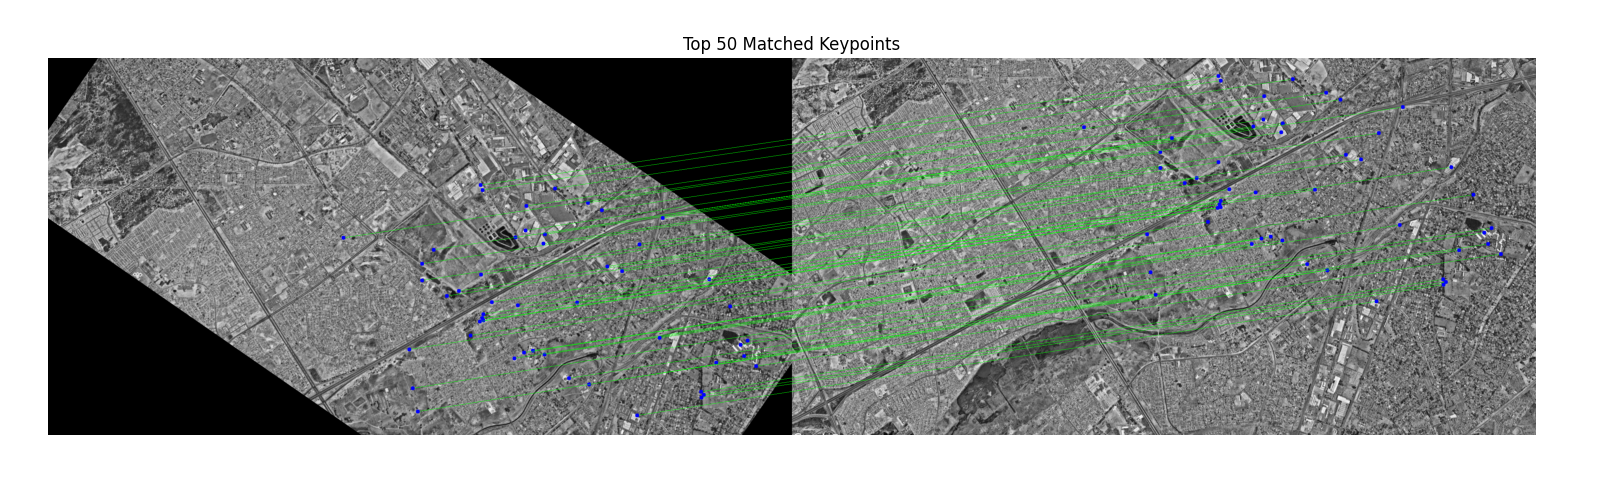
\includegraphics[width=0.94\textwidth]{./Chapter 2/litfigs/matche.png}
    \caption{Feature Detection and Matching}
    \label{fig:feature_detection}
\end{figure}





In this context, \textit{features} refer to both keypoints and descriptors, as each feature extraction method provides both components to facilitate effective image matching. The selection of feature extractors is guided by criteria such as accuracy, computational efficiency, robustness to diverse datasets, and the necessity for freely available tools, thereby excluding proprietary methods like SURF due to licensing fees. Additionally, chosen methods must hold credibility within the field, given their application in safety-critical UAV navigation systems.

The feature detectors selected for this system—\textbf{ORB}, \textbf{AKAZE}, and \textbf{SuperPoint with LightGlue}—offer a range of performance characteristics, balancing accuracy, computational efficiency, and machine learning integration. These extractors are further elaborated in the subsequent sections.

\subsubsection{ORB (Oriented FAST and Rotated BRIEF)}

\textbf{ORB} combines the \textbf{FAST} keypoint detector with the \textbf{BRIEF} descriptor, enhanced for rotation invariance. \textbf{FAST} rapidly identifies keypoints by analyzing pixel intensity differences in a circular region around each candidate point. Once detected, \textbf{BRIEF} encodes the local image patch into a binary string through intensity comparisons. ORB introduces rotational invariance by aligning keypoints based on their dominant orientation before descriptor computation. This enhancement makes ORB both fast and robust to scale and in-plane rotation, although it may struggle with repetitive textures or complex lighting variations \cite{opencv_orb_tutorial}.

\subsubsection{AKAZE (Accelerated-KAZE)}

\textbf{AKAZE} constructs a nonlinear scale space using diffusion-based filtering, capturing finer image details more effectively than linear methods. It detects keypoints by assessing local contrast with a specialized adaptive filter, enabling the identification of subtle features that simpler detectors might miss. The \textbf{Modified Local Difference Binary (MLDB)} descriptor encodes the neighborhood of each keypoint into a binary vector based on pixel intensity differences. While AKAZE is both fast and compact, its performance can be sensitive to detection thresholds across different environments, potentially affecting its robustness in varied operational contexts \cite{opencv_akaze}. 

\subsubsection{SuperPoint with LightGlue}

\textbf{SuperPoint} is a deep learning-based keypoint detector and descriptor that leverages convolutional neural networks (CNNs) to identify and describe keypoints in a single forward pass. Pre-trained on extensive image datasets, SuperPoint excels at recognizing stable and distinctive keypoints under varied conditions \cite{rpaultrat2023superpoint}. However, its performance may degrade on datasets significantly different from its training data. Pairing SuperPoint with \textbf{LightGlue}, a machine-learning-based matcher, enhances matching accuracy through advanced graph-based techniques \cite{cvg2023lightglue}. Despite their high accuracy, SuperPoint and LightGlue are computationally intensive, necessitating GPU acceleration for real-time applications.



% -----------------------------------------------------------------------------------------------------------------------------------


\subsection{Feature Matching}

Feature matching establishes correspondences between keypoints in different images based on descriptor similarity. After identifying these correspondences, ambiguities and low-quality matches are removed to retain only the most reliable matches, which are then used to estimate transformations such as translation and rotation. This filtering ensures that transformation estimations are based solely on mutual information between images, enhancing the accuracy and reliability of the navigation system.

Each matcher generates a list of potential matches along with their similarity scores, quantified using a descriptor-space distance metric. These scores are instrumental in determining the quality of the matches and play a crucial role in the subsequent filtering and transformation estimation processes.

Feature matching involves two primary components: the choice of matching technique to acquire potential matches and the search technique that determines which of these matches to retain. 

\subsubsection{Types of Feature Matching Techniques}

The following match acquisition techniques are commonly employed in feature-based navigation systems:

\textbf{Brute-Force Matcher (BFMatcher)}: The Brute-Force Matcher compares each feature in one image with every feature in the second image, ensuring the best possible match based on descriptor similarity. While this guarantees high accuracy, it is computationally expensive, especially with large numbers of keypoints, making it less suitable for real-time applications without optimization \cite{opencv_bfmatcher}.

\textbf{Fast Library for Approximate Nearest Neighbours (FLANN)}: FLANN accelerates the nearest neighbour search in high-dimensional descriptor spaces using algorithms such as KD-trees or hierarchical clustering. This approximate matching approach offers significant speed improvements with minimal loss in accuracy, making it ideal for real-time applications with extensive datasets \cite{opencv_flann_tutorial}.

\textbf{LightGlue}: Leveraging deep learning, LightGlue improves matching accuracy by employing advanced graph-based techniques to establish more reliable correspondences. Although highly effective, its structure necessitates the use of other neural network-based feature extractors like SuperPoint to realize its full potential \cite{cvg2023lightglue}. The enhanced accuracy comes at the cost of increased computational demands, requiring GPU acceleration for optimal performance.

The following search techniques are commonly used to filter matches and retain only the most reliable correspondences:

\textbf{Radius Search}: This method retains matches within a specified distance in descriptor space, effectively filtering out weaker matches. However, it does not guarantee a fixed number of matches per keypoint, leading to inconsistent results \cite{opencv_matcher_tutorial}.

\textbf{K-Nearest Neighbours (KNN) Matching}: KNN matching retains the top K matches for each keypoint, allowing the application of post-filtering techniques such as Lowe’s ratio test to eliminate ambiguous matches \cite{opencv_matcher_tutorial}.

\textbf{Vanilla Matching}: Vanilla matching returns the single best match for each keypoint based on the closest descriptor distance. It is a subset of KNN matching with K=1, offering simplicity and ease of implementation \cite{opencv_matcher_tutorial}.


Further, these matches are filtered using multiple techniques to ensure accuracy; this is discussed in the optimization techniques section.




% -----------------------------------------------------------------------------------------------------------------------------------


\subsection{Image Similarity Computation}

Image similarity computation is a pivotal component of UAV navigation systems that rely on reference images for accurate localization and pose estimation. Effective similarity measures ensure efficient processing of extensive image datasets and facilitate precise transformation estimations, which are essential for reliable navigation.

\subsubsection{Proximity-Based Techniques}

To achieve real-time performance, the search space is reduced to images within the proximity of UAV's last known location, filtering images within a static or dynamic radius. While this method is highly efficient, it does not account for potential deviations from the expected flight path or the presence of poor-quality reference images. This limitation implicates that this measure cannot be used as the sole basis for image similarity computation, necessitating the integration of additional techniques for comprehensive assessment.

\subsubsection{Global Matching Techniques}

Direct methods estimate planar transformations by comparing entire image pixel intensities and minimizing differences through optimization techniques like gradient descent. This single-layer processing allows for efficient analysis of multiple images and a comprehensive understanding of image similarity within the global context, making direct methods suitable for scenarios with minor viewpoint changes. However, relying on full pixel usage reduces accuracy in cases of significant transformations due to increased sensitivity to noise and the assumption of smooth, incremental UAV movements. Direct methods are best suited for applications that aim to estimate similarity across large image sets. These methods necessitate rotational alignment of images to eliminate bias introduced by orientation discrepancies \cite{GlobalLocal2023}. The following subsections detail the primary global matching techniques employed in this system to compute similarity scores.


\textbf{Cross-Correlation}

Cross-correlation measures similarity by sliding one image over another and computing the sum of pixel-wise multiplications at each position. The peak value signifies the best alignment, and its magnitude indicates the confidence level of the similarity. Higher confidence values reflect greater similarity between the images. While straightforward to implement, cross-correlation is sensitive to noise and illumination changes, which can compromise the reliability of the similarity measure \cite{sharma2022crosscorrelation}.

\textbf{Histograms}

Histogram comparison assesses similarity by analyzing the distribution of pixel intensities within each image. Typically, each image's histogram is divided into 256 intensity bins, and similarity is quantified using metrics such as Chi-Square or Bhattacharyya distance. This method emphasizes global color and brightness distributions but neglects spatial information, making it less effective for nuanced structural differences \cite{rosebrock2014comparehistograms}.

\textbf{Structural Similarity Index (SSIM)}

SSIM evaluates similarity by decomposing images into luminance, contrast, and structure components. It computes local statistics within small windows and integrates them into a single similarity score that mirrors perceived image quality. SSIM effectively captures structural information like edges and textures, aligning closely with human visual perception. Although slightly more computationally expensive than the former methods, it is robust to varied conditions \cite{rosebrock2017imagedifference}. An illustration of SSIM is shown in Figure \ref{fig:ssim} from \cite{rosebrock2017imagedifference}.

\begin{figure}[H]
    \centering
    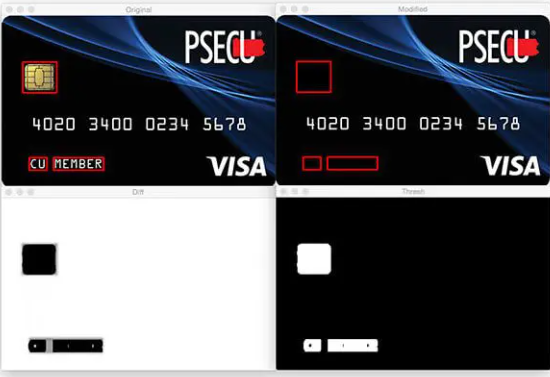
\includegraphics[width=0.65\textwidth]{./Chapter 2/litfigs/SSIMeg.png}
    \caption{Structural Similarity Index (SSIM)}
    \label{fig:ssim}
\end{figure}

\textbf{Local Detectors Conversion}

Although not inherently a global matching technique, local feature matching can be adapted to achieve a global understanding of image similarity. This involves identifying and matching keypoints in both images and assessing the overall number of good matches. However, this approach alone does not ensure an even distribution of matches across the entire image, potentially leading to biased, localized similarity assessments. To mitigate this, a grid matching technique is employed, dividing the image into grids and limiting the number of matches per grid. Although the most computationally intensive, this method enhances robustness against distortions and rotations by ensuring a uniform distribution of matches across the image.



% -----------------------------------------------------------------------------------------------------------------------------------


\subsection{Planar Transformation Estimators}

Feature-based methods extract and match keypoints from both reference and real-time images, often incorporating outlier removal stages \cite{GlobalLocal2023}. By focusing on distinctive features rather than every pixel, these methods excel in handling large viewpoint changes and rotations, enabling more precise transformation inference. This targeted approach enhances computational efficiency and robustness to environmental distortions, though it requires careful management to avoid performance degradation from variation in the number of extracted feature points. Feature-based methods are preferable for applications demanding high accuracy and adaptability in complex environments \cite{nguyen2018}. These feature-based transformations enable precise updates to the UAV's pose and location, facilitating accurate navigation and control. The following subsections outline the primary planar transformations employed in this system.


\subsubsection{Affine Transformation}

Affine transformation captures translation, rotation, scaling, and shear, providing six degrees of freedom. It is represented by a  \(2 \times 3\) matrix that maps points from one plane to another while preserving lines and parallelism. Affine transformations are computed by estimating the affine transformation matrix between two sets of corresponding points using OpenCV's \texttt{estimateAffine2D} function \cite{opencv_warp_affine}. While versatile, the inclusion of scaling and shear can introduce unnecessary complexity for scenarios where only rotation and translation are relevant, potentially impacting the accuracy of transformation estimations.

\subsubsection{Rigid Transformation Estimation (SVD)}

Rigid transformation preserves the shape and size of objects by estimating only rotation and translation, excluding scaling and shear. Represented by a  \(2 \times 3\) matrix, rigid transformation ensures orthogonality in the rotation component. Utilizing Singular Value Decomposition (SVD), this method minimizes the least-squares error between two point sets. The process involves: computing the weighted centroids of both point sets, centering the points by subtracting their respective centroids, calculating the covariance matrix of the centered points, performing SVD on the covariance matrix to derive the rotation matrix, and determining the translation vector based on the centroids. The resulting \(2 \times 2\) rotation matrix and \(2 \times 1\) translation vector are combined to form the rigid transformation matrix. Rigid transformation is computationally efficient and well-suited for applications requiring only rotation and translation \cite{sorkine2017least_squares}.


\subsubsection{Partial Affine Transformation}

Partial affine transformation simplifies the full affine model by focusing solely on translation, rotation, and uniform scaling, offering four degrees of freedom. This transformation is also represented by a \(2 \times 3\) matrix, similar to the affine transformation but without shearing and with reduced, uniform scaling. By limiting scaling to be uniform, partial affine transformation reduces potential distortions and maintains simplicity, making it ideal for scenarios where only rotation and translation are significant \cite{opencv_warp_affine}.

\subsubsection{Homography Transformation}

Homography transformation accounts for translation, rotation, scaling, shear, and perspective distortion, providing eight degrees of freedom. It is represented by a \(2 \times 3\) matrix and is estimated using OpenCV's \texttt{findHomography} function, typically with RANSAC for outlier rejection \cite{opencv_homography}. While homography offers greater flexibility in modeling complex transformations, its additional degrees of freedom can introduce unnecessary errors and computational overhead for simpler applications that only require rotation and translation. Consequently, homography is reserved for scenarios necessitating comprehensive transformation modeling beyond rotation and translation.


% -----------------------------------------------------------------------------------------------------------------------------------
\subsection{Optimization Techniques}

Optimizing parameter sets is essential for enhancing the performance and robustness of the UAV navigation system. These optimization techniques aim to refine the accuracy and reliability of the point cloud used for transformation estimation by effectively filtering out erroneous matches and improving transformation accuracy. The following subsections detail the primary optimization methods employed in this system.

\subsubsection{Random Sample Consensus (RANSAC) for Planar Transformation}

RANSAC is a robust estimation technique used to estimate planar transformations by iteratively selecting random subsets of point correspondences to fit a model and identify inliers \cite{fisher2002ransac}. The process involves randomly selecting a minimal subset of point pairs, estimating the transformation model (e.g., affine or homography) based on the selected subset, determining the number of inliers that fit the estimated model within a predefined threshold, and repeating the process for a set number of iterations or until a sufficient inlier ratio is achieved. This approach is highly effective in datasets with significant outliers, focusing on finding a model that best fits the largest subset of inliers. However, due to its iterative nature and the need to sample repeatedly, RANSAC can result in increased runtime, particularly in larger datasets or when dealing with numerous outliers \cite{fisher2002ransac}.

\subsubsection{Local Maxima Extrema Density Selection (LMEDS) for Planar Transformation}

LMEDS is a keypoint selection method designed to prioritize areas of high feature density by identifying local maxima as keypoints for matching \cite{farin2005video}. This technique involves analyzing the image to identify regions with high feature density, selecting keypoints located at local maxima within these dense regions, and filtering out less significant keypoints to reduce redundancy and improve match quality. By concentrating on areas with high feature concentration, LMEDS ensures that keypoints represent the most distinctive and informative regions of the image, enhancing both accuracy and performance by reducing redundant keypoints and improving match quality, particularly in areas with high feature variability.

\subsubsection{Lowe's Ratio Test}

Lowe's ratio test is a filtering technique used to eliminate ambiguous or false keypoint matches by comparing the distance of the best match to the second-best match \cite{bian2020gms}. For each keypoint match, the ratio of the distance of the best match to that of the second-best match is calculated, and the match is retained if this ratio is below a predefined threshold. A lower ratio indicates that the best match is significantly better than the alternatives, thereby increasing the likelihood of the match being correct. An example of Lowe's ratio test filtration are showed in figure \ref{fig:lowes1} and \ref {fig:lowes2} from \cite{bian2020gms}. 


\begin{figure}[H]
    \centering
    \begin{subfigure}[b]{0.36\textwidth}
        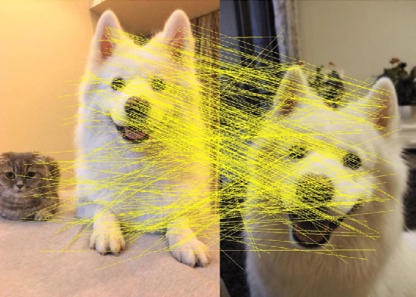
\includegraphics[width=\textwidth]{./Chapter 2/litfigs/lowes1.png}
        \caption{Without Lowe's Ratio Test}
        \label{fig:lowes1}
    \end{subfigure}
    \hfill
    \begin{subfigure}[b]{0.364\textwidth}
        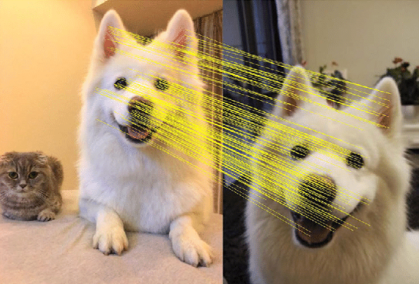
\includegraphics[width=\textwidth]{./Chapter 2/litfigs/lowes2.png}
        \caption{High Ratio Test}
        \label{fig:lowes2}
    \end{subfigure}
    \caption{With Lowe's Ratio Test}
    \label{fig:lowes}
\end{figure}


\subsubsection{Standard Deviation Filtering}

Standard deviation filtering involves computing an average for the dataset, typically the mean or median, and removing matches that deviate significantly from this average. This technique is simple to implement but has the ability to generalize well across datasets due to its relative nature. 

\subsubsection{N-Match or Absolute Thresholding}
N-match thresholding involves setting a threshold that allows only a specific number of matches with the smallest descriptor distances to be retained. Absolute thresholding filters matches based on a fixed distance in descriptor space. Only matches that meet or fall below this predefined distance threshold are retained, ensuring that only sufficiently similar matches are used in the transformation estimation process. These methods primarily suffer from difficulty in setting the threshold, which is often extremely sensitive to dataset variations and method parameters.
